%% LyX 2.0.0 created this file.  For more info, see http://www.lyx.org/.
%% Do not edit unless you really know what you are doing.
\documentclass[english]{article}
\usepackage[T1]{fontenc}
\usepackage[utf8]{luainputenc}
\usepackage{graphicx}

\makeatletter

%%%%%%%%%%%%%%%%%%%%%%%%%%%%%% LyX specific LaTeX commands.
%% Because html converters don't know tabularnewline
\providecommand{\tabularnewline}{\\}
%% A simple dot to overcome graphicx limitations
\newcommand{\lyxdot}{.}


%%%%%%%%%%%%%%%%%%%%%%%%%%%%%% Textclass specific LaTeX commands.
\newenvironment{lyxlist}[1]
{\begin{list}{}
{\settowidth{\labelwidth}{#1}
 \setlength{\leftmargin}{\labelwidth}
 \addtolength{\leftmargin}{\labelsep}
 \renewcommand{\makelabel}[1]{##1\hfil}}}
{\end{list}}

\makeatother

\usepackage{babel}
\begin{document}
File System Operations:

\textbf{1. Size of File Cache:}
\begin{enumerate}
\item Prediction :- Size of file cache should be some fraction of the memory
(RAM) in the system. Kernel reserves some memory ( in terms of data
structures it uses and say by the paging dameon). Bottomline, we expect
it to be some fraction of RAM on system. 
\item Experiment : - The idea is to bring all the pages of the file in file
cache and read it again. As long as the entire file can fit in the
file cache, we will see similar per block read numbers. But as soon
as we read a file, some pages will have to be fetched from disk and
not the file cache. Thus we will see a bump in the read numbers. The
following steps describe the experiment: 

\begin{itemize}
\item Step1: Read a file of say size 100M sequentially. This will bring
in the entire file in the file cache
\item Step2: Read the same file again, measure the time to read it
\item Step 3: Increase the file size, repeat Step 1 and Step 2. 
\item Step 4: Continue Step 3, after a while when file size is larger than
file cache, the per block read time will increase
\item Step 5: Plot per block read time as function of file size
\end{itemize}
\end{enumerate}
3. Results: 

\begin{tabular}{|c|c|c|}
\hline 
File Size (MB) & CPU Cycles / MB & Time (ms)\tabularnewline
\hline 
\hline 
150 & 1424800 & 50\tabularnewline
\hline 
200 & 4325000 & 1.6\tabularnewline
\hline 
250 & 7284000 & 2.7\tabularnewline
\hline 
300 & 35256000 & 13.1\tabularnewline
\hline 
350 & 34762000 & 12.9\tabularnewline
\hline 
400 & 30081000 & 11.1\tabularnewline
\hline 
450 & 36080000 & 13.4\tabularnewline
\hline 
500 & 28269000 & 10.5\tabularnewline
\hline 
550 & 29327000 & 10.9\tabularnewline
\hline 
600 & 27972000 & 10.4\tabularnewline
\hline 
650 & 31478000 & 11.7\tabularnewline
\hline 
700 & 30541000 & 11.3\tabularnewline
\hline 
\end{tabular}

\textbf{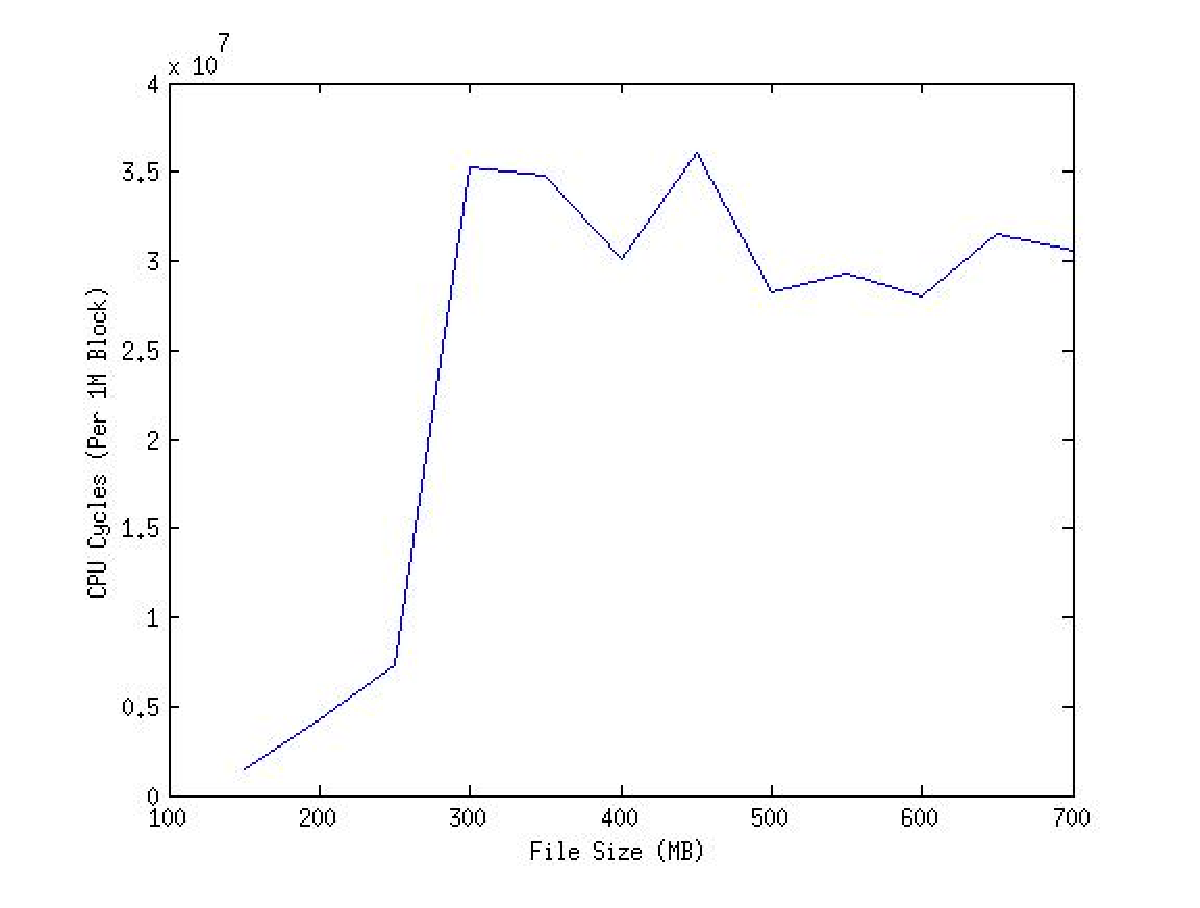
\includegraphics[scale=0.5]{/home/vineetm/Documents/res4_1}}

4. Analyis : The graph clearly shows that as file size reaches 300M
we see a bump in the average read time. The RAM in our system is close
to 500M, thus file cache of 300M seems to be a pretty convincing result.

\textbf{File Read time:}
\begin{enumerate}
\item Prediction :- We expect file read time to be worse for a random read
when compared to a sequential read (when we don't use file cache).
This is beacuse sequential read on disk involves less seek time.
\item Experiment :-

\begin{enumerate}
\item Open a file in O\_DIRECT mode, this ensures that no file cache is
used
\item Read the file sequentially, measure time
\item Read the file randomly (using preads) and generating a random offset,
measure time
\item Repeat (a) - (c) by increasing the size of file\end{enumerate}
\begin{lyxlist}{00.00.0000}
\item [{%
\begin{tabular}{|c|c|c|c|c|}
\hline 
File Size(MB) & Sequential (CPU Cycles)(Million) & Sequential Time(ms) & Random (CPU Cycles) & Random(ms)\tabularnewline
\hline 
\hline 
32 & .584 & 0.2163 & .597 & 0.2212\tabularnewline
\hline 
64 & .587 & 0.2212 & .598 & 0.2218\tabularnewline
\hline 
150 & .591 & 0.2190 & .601 & 0.2229\tabularnewline
\hline 
200 & .591 & 0.2192 & .619 & 0.2296\tabularnewline
\hline 
250 & .613 & 0.2273 & .645 & 0.2391\tabularnewline
\hline 
300 & .616 & 0.2285 & .615 & 0.2279\tabularnewline
\hline 
400 & .588 & 0.2179 & .609 & 0.2257\tabularnewline
\hline 
 &  &  &  & \tabularnewline
\end{tabular}}]~
\end{lyxlist}
\item 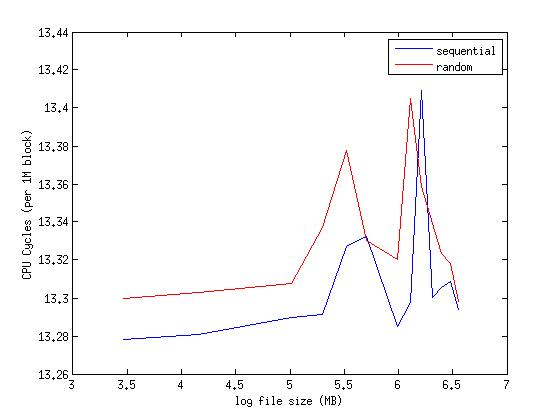
\includegraphics[scale=0.5]{/home/vineetm/Documents/res4_2}
\item Analysis : It seems from the graph that sequential writes work little
bit better than random writes.
\end{enumerate}
\textbf{3. Remote file read time}

1. Prediction : - Network penalty is going to overshadow any difference
between sequantial and random read. Also, we predict that network
penalty is going to be very high.

2. Experiment
\begin{itemize}
\item Continuing the setup of last experiment, start a nfs server and share
a folder across network
\item Mount the shared folder on a client
\item Read files in increasing order of size from the client, measure time
to do sequential as well as random read
\end{itemize}
3. Results:

\begin{tabular}{|c|c|c|c|c|}
\hline 
File Size(MB) & CPU Cycles - Sequential(Million) & Time(s)  & CPU Cycles- Random (M) & Time\tabularnewline
\hline 
\hline 
32 & 2555 & 0.9465 & 2885 & 1.0686\tabularnewline
\hline 
64 & 2456 & 0.9099 & 2617 & 0.9694\tabularnewline
\hline 
150 & 2933 & 1.0861 & 2673 & 0.9898\tabularnewline
\hline 
200 & 2830 & 1.0485 & 2816 & 1.0430\tabularnewline
\hline 
250 & 3012 & 1.1171 & 2915 & 1.0795\tabularnewline
\hline 
300 & 2569 & 0.9515 & 2837 & 1.0509\tabularnewline
\end{tabular}

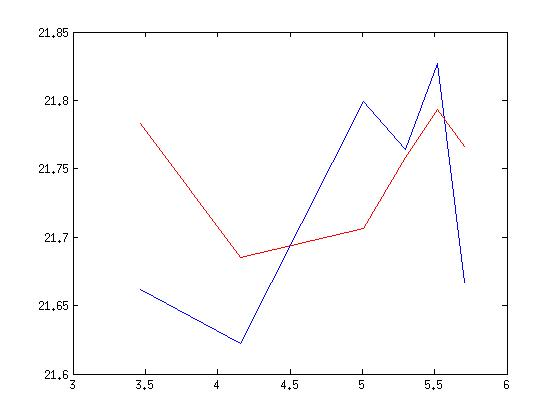
\includegraphics[scale=0.5]{/home/vineetm/Documents/res4_3}

4. Analysis : Network Penalty seems to be of the order of 0.8 seconds.
Read time for one block was in milliseconds, but over NFS this is
in terms of seconds. Also, its interesting to note that affect of
random read has been nullified.

\textbf{4. Measuring contention:}

We are measuring the effect on read operation time when number of
processes reading potentially different files in the same filesystem
(hence the same 2disk) increase.
\begin{enumerate}
\item Prediction - We expect read time to increase as number of processes
in the system (doing some read operation) increase. As number of processes
increase they will cause the disk head to move more and thus from
the perspective of one process seek time will increase - even when
it is doing a sequential access. However there might not be a direct
correlation with number of processes. All we predict is that we are
going to see increase in read time as there are other processes reading
on the disk.
\item Experiment \end{enumerate}
\begin{itemize}
\item Set block size as 4K. Note that this does not need to be 4K, but when
measuring time per block size, we would make this block size as fixed
so that we are comparing the same quantities
\item Create a file of 100M. Read it for a fixed number of iterations (Do
repeated reads on this file)
\item Open all files for this experiment using O\_DIRECT. This ensures that
we are not using file cache and are directly accessing disk
\item Measure time taken to read one block when 1 other process is reading
a file (this file is differnt than first process
\item Measure time to read when 2 processes are reading 2 different files
\item Continue this experiment by reading a file when 20 processes are running.
\item Compare results
\end{itemize}
3. Results

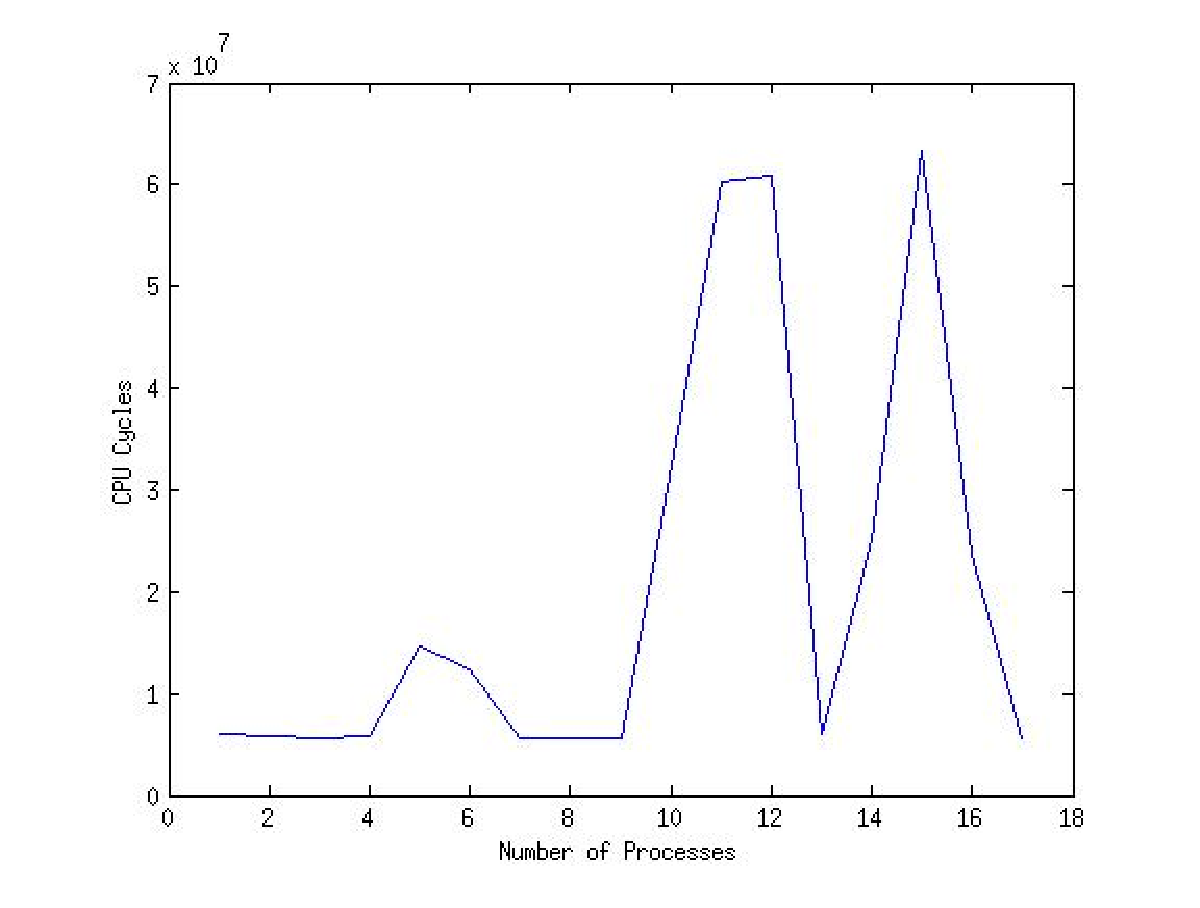
\includegraphics[scale=0.5]{/home/vineetm/Documents/res1}

4. Analysis

Graph shows that as number of processes increase the variations in
reading time increase too. Thus our original prediction that as more
processes try to read a file on sam disk, seek time should vary a
lot, seems correct
\end{document}
